\section[Características de SuperCollider]{Características importantes de SuperCollider y sus limitaciones}
\sectionmark{SuperCollider}
\label{sec:sc_features}

\appName~ha sido escrito enteramente en SuperCollider. Antes de entrar en detalles de su funcionamiento conviene describir brevemente algunas de las características estructurales de SuperCollider que se han tenido muy en cuenta a la hora de programar la aplicación.

\subsection{Orden de ejecución en el servidor}
En un sintetizador modular analógico no hay limitación alguna en el orden en el que se conecta sus módulos. Todos son independientes entre sí ya que se <<ejecutan>> al mismo tiempo. Cualquier señal de salida puede ser conectada a cualquier entrada. Esta es una de las características más interesantes y sugerentes de estos sintetizadores. En el manual de instrucciones de EMS Synthi VCS3 \cite{SynthiVCS3_brochure}  --antecesor del Synthi 100 y de características muy similares-- se invita al usuario a experimentar libremente con cualquier conexión. La posibilidad de que todo pueda ser conectado con todo hace de los sintetizadores modulares en general, y de los Synthi en particular, un banco de experimentación sonora sin precedentes.

Los sistemas informáticos actuales son multihilo, es decir, pueden ejecutar varias tareas a la vez. El tiempo de ejecución es repartido en todas ellas a velocidad suficiente como para crear en el usuario la ilusión de que ocurren las tareas simultáneamente, cuando en realidad solo una se lleva a cabo en un instante concreto. Los sintetizadores digitales aprovechan esta característica, pero sus módulos no se ejecutan simultáneamente, sino que siguen un orden preciso de ejecución entre ellos. En el caso de SuperCollider, cada \textit{Synth} en el servidor ocupa un lugar en una lista, la cual es ejecutada en orden a la frecuencia de audio (\textit{audio rate}). Puesto que todos los módulos de \appName~están construidos a base de \textit{Synths}, no será raro que la salida de uno de ellos sea conectada a la entrada de otro que ya ha sido ejecutado en el ciclo presente. El contenido de los \textit{busses} de audio es eliminado al terminar un ciclo completo, por lo que ninguna señal llegará al módulo de destino. La figura \ref{fig:sc_server} representa esta característica de unidireccionalidad en el orden de ejecución de los nodos presentes en el servidor. Ningún \texttt{Synth} podrá enviar señal alguna a otro situado a su izquierda (el orden de ejecución es de izquierda a derecha en esta representación).

\begin{figure}
	\centering
	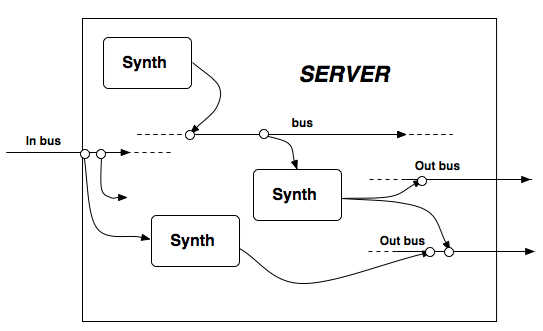
\includegraphics[width=0.7\textwidth]{images/sc_server}
	\caption[Orden de ejecución en el servidor de SuperCollider]{Orden de ejecución en el servidor de SuperCollider. Cada ciclo de audio los \texttt{Synths} presentes en el servidor son ejecutados en orden (de izquierda a derecha en esta respresentación). Ninguna información puede viajar por los \textit{busses} en sentido contrario, ya que su contenido es eliminado tras la finalización de cada ciclo.}
	\label{fig:sc_server}
\end{figure}

Existe un \textit{UGen} que permite obtener información de ciclos pasados de los \textit{busses}. Se trata de \texttt{InFeedback}. La limitación frente a \texttt{In} es que la señal que recibe es la correspondiente a un ciclo de control previo. Aunque en la mayoría de los casos esto no tiene mayor importancia, es una característica importante a tener en cuenta, especialmente cuando se produce un \textit{feedback} en la señal, ya que su comportamiento distará mucho del que puede tener un sistema analógico. 

\subsection{\textit{Audio rate} y \textit{control rate}}
No todo ocurre a la misma velocidad en SuperCollider. La producción de señales de audio requiere de la creación de un número de muestras por segundo igual a la <<tasa de audio>>. Pero no siempre es necesaria una demanda tan alta de computación. En el caso de los efectos como curvas relativamente lentas en los cambios de los parámetros sonoros pueden realizarse con una tasa mucho menor. Por ejemplo, un \textit{glissando} frecuencial entre 100 Hz y 1000 Hz de un segundo de duración, no necesita tener una resolución similar a la <<tasa de audio>>\footnote{Sin entrara aquí en detalles, la frecuencia mínima de audio utilizada un sistema digital normal es de 44.1 KHz, la correspondiente a un CD de audio estándar.}. Es posible realizarlo a una tasa (<<de control>>) bastantes veces menor a la de audio sin verse afectado auditivamente el resultado sonoro. Por defecto, la tasa de control en SuperCollider es 64 veces menor que la de audio.

Existe una clara analogía entre una señal de audio analógica y \textit{audio rate}, así como entre una señal de voltaje y \textit{control rate}. En una primera aproximación, podría parecer obvio que las señales de voltaje del Synthi 100 pueden ser emuladas digitalmente a la tasa de control. El problema de una decisión así es que limita considerablemente el uso que podemos hacer con esta señales <<de control>>. En un sintetizador analógico, una señal de control de voltaje puede ser utilizada como señal de audio y viceversa. No hay ninguna diferencia real entre ambos tipos de señal, más allá de una división puramente funcional. No hay ninguna razón que nos obligue a limitar las compotentes frecuenciales de una señal de voltaje en un sintetizador analógico. Por esta razón, \appName\ prescinde por completo de las señales en <<tasa de control>>. Todas las señales en la aplicación son del mismo tipo, con <<tasa de audio>>. Esto es posible, evidentemente, gracias a la capacidad de computación de los ordenadores modernos. A cambio de eficiencia se gana en versatilidad y, por supuesto, en aproximación al funcionamiento de un sintetizador modular.


\subsection{Los \textit{Synths} ocupan recursos...}
Puede resultar una obviedad decir que tanto los \textit{Synths} como los \textit{busses} digitales ocupan memoria y tiempo de ejecución, pero cuando estos elementos se empiezan a contar por miles, como en el caso de \appName, este es un factor que puede comprometer la eficiencia y la escalabilidad de la aplicación.

En el diseño de \appName~ se ha prestado una especial atención en la eficiencia. \textit{Sclang} es un lenguaje de alto nivel e interpretado \textit{just in time}, por lo que necesita de un consumo de recursos de computación mayor que el de lenguajes de bajo nivel y compliados, como ocurre con C o C\texttt{++}. Los \textit{Synth} son básicamente unas funciones que se ejecutan una vez cada ciclo de audio. Si cada módulo tiene entre uno y cinco \textit{Synths} y otro cada nodo de las matrices, contaríamos por varios miles los \textit{Synths} que se ejecutarían al mismo tiempo, lo cual comprometería el correcto funcionamiento del sistema en su conjunto.

Para que esto no ocurra, todos los \textit{Synths} están <<pausados>> por defecto. Solo se ejecutan cuando cumplen ciertas condiciones. Cada módulo y cada \textit{Synth} tiene implementadas unas condiciones distintas para ejecutarse, pero, en términos generales, si la salida de un módulo no está conectada en la matriz a otro modulo, no producirá ninguna señal hasta que se <<le comunique>> que está conectado. Lo mismo ocurre si su salida tiene ganancia $0$. Otros factores, en función de las características de cada módulo, se sopesan a la hora de decidir su pausa o ejecución, como si recibe o no alguna entrada (en el caso de un efecto) o de si se espera que siga ejecutándose incluso sin entradas y salidas (el módulo \textit{Echo}, \ref{sec:echo}), para que siga procesándose la información que almacena temporalmente en su \textit{buffer}. 


\subsection{\textit{Aliasing}}
Esta es una característica propia de cualquier sistema de audio digital, y que más pronto que tarde aparece como un obstáculo en la emulación de la síntesis analógica ya que esta última es ajena a esta característica.

\begin{figure}
	\centering
	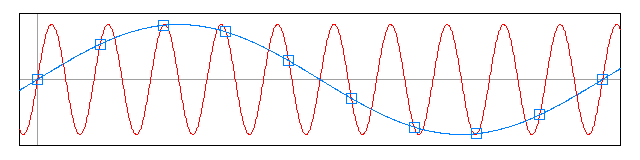
\includegraphics[width=0.9\textwidth]{images/aliasing}
	\caption[Gráfica de \textit{aliasing}]{Gráfica de aliasing. (CC BY-SA 3.0,\\ \href{https://commons.wikimedia.org/w/index.php?curid=275973}{\texttt{https://commons.wikimedia.org/w/index.php?curid=275973}})}
	\label{fig:aliasing}
\end{figure}

Cuando una señal senoidal periódica de frecuencia $f$ es muestreada a una frecuencia $s$ mayor que $f/2$, la señal reconstruida con dichas muestras corresponde a una frecuencia inferior a $f$. Para evitar este efecto en señales producidas digitalmente, la frecuencia de muestreo ha de ser al menos $2s$. Este es el <<criterio de Nyquist>>, en honor a su descrubridor. 

La figura \ref{fig:aliasing} muestra gráficamente este proceso. En rojo se representa la señal original, y en azul, la señal reconstruida a partir  de la muestras dibujadas como cuadrados. La frecuencia de la señal azul es mucho menor que la que se pretende reproducir. Solo una frecuencia mayor de muestreo (mayor densidad de cuadrados azules en la figura), al menos la mitad que la frecuencia de la señal roja, permitiría que la señal azul conservara la frecuencia.

Esta característica de las señales digitales no es compartida por los sintetizadores analógicos, razón por la cual se convierte en no deseable a la hora de emularlos. SuperCollider posee un gran abanico de \textit{UGens} cuya implementación intenta minimizar este efecto. Un criterio importante a la hora de elegir entre varios \textit{UGens} en el diseño de los \textit{Synths} de los módulos de Synthi 100 ha sido el que incorporasen algún tipo de sistema \textit{antialiasing}. Aun así, es impredecible el uso que se puede hacer de \appName: una simple frecuencia modulada producida con dos generadores sinusoidales producirá fácilmente \textit{aliasing}, ya que las frecuencias laterales producidas frecuentemente incumplirán el criterio de Nyquist.

La única forma efectiva y práctica de limitar la presencia de \textit{aliasing} es aumentar en la medida de lo posible la tasa de audio (\textit{sample rate}). Aun así, es probable encontrar combinaciones de módulos y sus parámetros que superen el límite de Nyquist, por alto que este sea.




